\documentclass[10pt]{beamer}

\usetheme[progressbar=frametitle]{metropolis}

\usepackage{appendixnumberbeamer}
\usepackage{booktabs}
\usepackage[scale=2]{ccicons}
\usepackage{pgfplots}
\usepgfplotslibrary{dateplot}
\usepackage{xspace}
\usepackage{graphicx}
\usepackage{subcaption}

\newcommand{\themename}{\textbf{\textsc{metropolis}}\xspace}

\title{Authorship Verification}
\subtitle{Project Outside Course Scope}
% \date{\today}
\date{}
\author{Magnus Stavngaard}
\institute{University of Copenhagen}
% \titlegraphic{\hfill\includegraphics[height=1.5cm]{logo.pdf}}

\begin{document}

\maketitle

\begin{frame}[fragile]{Introduction}

    \begin{itemize}
        \item Authorship Verification is determining whether the author of an
            unknown text is the same as the author of a known text.
        \item We explored methods for Authorship Verification.
        \item Use data from PAN 2013 and PAN 2015 competitions.
        \item PAN 2013 has average of 1038 words per author.
        \item PAN 2015 has average of 460 words per author.
    \end{itemize}

\end{frame}

\begin{frame}[fragile]{Delta Method}
    \begin{itemize}
        \item Distance based.
        \item Use the imposter method for authorship verification.
        \item Manhattan distance and word frequencies only.
        \item Cross validation to choose number of imposters and number of word
            frequencies.

        \begin{table}
        \begin{tabular}{cc}
            \textbf{PAN 2013} & 300 most frequent words and 4 imposters. \\
            \textbf{PAN 2015} & 200 most frequent words and 1 imposter.
        \end{tabular}
        \end{table}
    \end{itemize}
\end{frame}

%\begin{frame}[fragile]{Delta Method}

    %\begin{itemize}
        %\item Manhattan distance based approach using only word frequencies.
        %\item Set of imposter authors are chosen besides the author we are
            %verifying.
        %\item The author with the closest text is reported as the author.
        %\item Number of different word frequencies and imposter set size has to
            %be chosen.
    %\end{itemize}

%\end{frame}

%\begin{frame}[fragile]{Delta Method Implementation}

    %\begin{itemize}
        %\item Chose number of different word frequencies and imposter set size
            %via cross validation.
        %\item Number of different words vary from 100 to 500 and imposter set
            %size from 1 to 10.
        %\item The best results on PAN 2013 were 300 most frequent word
            %frequencies and an imposter set size of 4.
        %\item The best results on PAN 2015 were 200 most frequent word
            %frequencies and an imposter set size of 1.
    %\end{itemize}

%\end{frame}

\begin{frame}[fragile]{Generalising Random Forest}

    \begin{itemize}
        \item Based on a Universal Background Model (UBM) that describes a
            generic text not written by any specific author.
        \item The generic text is used to encode the feature vectors of other
            texts.

            \begin{equation}
                R_k = \frac{(A_k - U_k)^2 + 1}{(B_k - U_k)^2 + 1}
            \end{equation}
        %\item Features will be encoded such that features closer to the known
            %text of an author is between 0 and 1 and features closer to the UBM
            %is between 1 and $\infty$.
        \item Hope is that the random forest will learn which features should be
            closer to the known text than UBM for an unknown text to be written
            by the author of the known text.
        \item Another encoding,

            \begin{equation}
                R_k = A_k - U_k
            \end{equation}
        \item We used the features,
            \begin{itemize}
                \item 50 word n-grams for $n \in \{1, \dots, 5\}$.
                \item 50 character n-grams for $n \in \{2, \dots, 5\}$.
                \item 50 POS-tag n-grams for $n \in \{2, \dots, 5\}$.
                \item 5 special character n-grams for $n \in \{2, 3\}$.
            \end{itemize}
    \end{itemize}

\end{frame}

\begin{frame}[fragile]{Extended Delta Method}

    \begin{itemize}
        \item Different extensions to the Delta Method:
            \begin{itemize}
                \item Using different distance metrics/measures.
                \item Using different features than the frequencies of the most
                    frequent words.
            \end{itemize}
        \item We use two distance metrics Manhattan and Euclidean.
        \item Manhattan performed better than Euclidean.
        \item We tried 20 different feature combinations.
        \item Best features for PAN 2013 were the 100 most frequent character
            2-3-4-grams and the 300 most frequent word frequencies.
        \item Best features for PAN 2015 were the 20 most frequent special
            character 1-2-3-grams.
    \end{itemize}

\end{frame}

\begin{frame}[fragile]{Author Specific SVM}

    \begin{itemize}
        \item The imposter method.
        \item SVM classifier is trained with $n$ texts written by an author and
            $n$ texts from imposters.
        \item We tried two feature combinations. The first configuration
            consisted of the 500 most frequent character 3-4-5-grams, the 100
            most frequent word 3-4-grams and the 20 most frequent POS-tag
            2-3-4-grams. The second configuration is just the frequencies of
            the 300 most frequent words.
        \item We used an RBF kernel.
        \item Cross validation to find hyperparameters. Looked for $C \in
            \{10^{-2}, 10^0, \dots, 10^{10}\}$ and $\gamma \in \{10^{-9},
            10^{-7}, \dots, 10^3\}$.
        \item We performed leave one out cross validation for each author in
            training dataset independently and then used majority vote to find
            the actual hyperparamters. The best parameters for configuration 1
            were $C = 100$ and $\gamma = 0.00001$ and for configuration 2
            $C = 100$ and $\gamma = 0.001$.
    \end{itemize}

\end{frame}

\begin{frame}[fragile]{PAN 2013 Results}

    \begin{itemize}
        \item Delta Method Accuracy 0.62252.
        \item Extended Delta Method Accuracy 0.69909.
        \item Author Specific SVM Accuracy 0.77858.
        \item Obtained third place in the PAN 2013 competition.
    \end{itemize}

\end{frame}

\begin{frame}[fragile]{PAN 2015 Results}
    \begin{figure}
        \begin{subfigure}{.4\textwidth}
            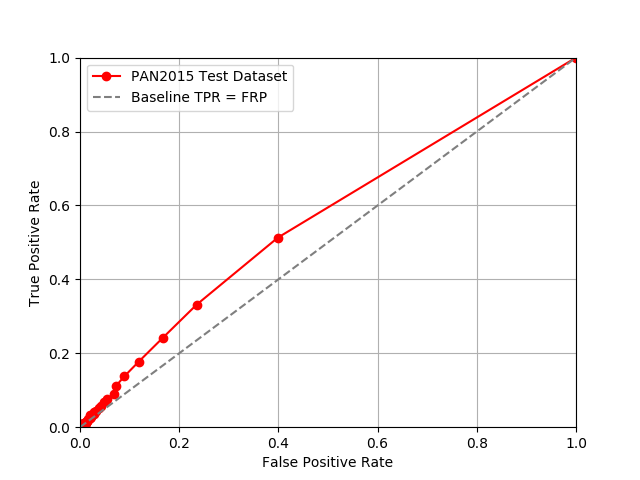
\includegraphics[width=\textwidth]{../../report/pictures/delta_method_roc.png}
            \caption{Delta Method ROC}
        \end{subfigure}
        \begin{subfigure}{.4\textwidth}
            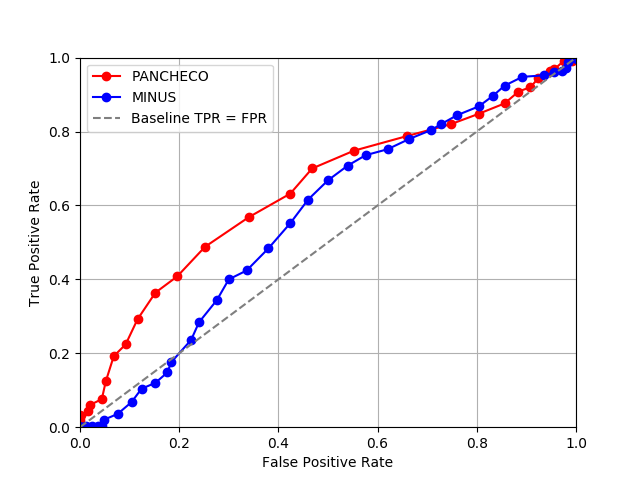
\includegraphics[width=\textwidth]{../../report/pictures/forest_roc.png}
            \caption{Generalising Random Forest ROC}
        \end{subfigure}
        \begin{subfigure}{.4\textwidth}
            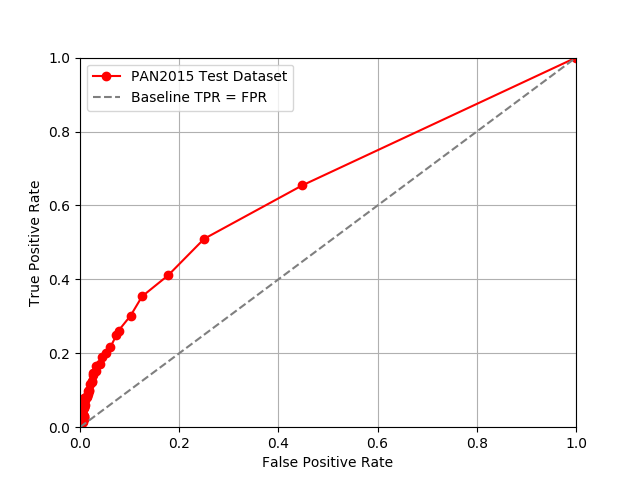
\includegraphics[width=\textwidth]{../../report/pictures/extended_delta_method_roc.png}
            \caption{Extended Delta Method ROC}
        \end{subfigure}
    \end{figure}
\end{frame}

\begin{frame}[fragile]{PAN 2015 Results}

    \begin{itemize}
        \item Delta Method Final Score 0.34201.
        \item Random Forest UBM 0.38576.
        \item Random Forest Minus 0.33183.
        \item Extended Delta Method 0.40383.
        \item Obtained 8th place in PAN 2015.
    \end{itemize}

\end{frame}

\begin{frame}[fragile]{Most Important Features}
    \begin{table}
        \centering
        \begin{tabular}{lll}
            \textbf{Feature Class} & \textbf{Feature}     & \textbf{Importance Score} \\
            \hline
            char-4-gram            & 'for '               & 0.01230                   \\
            char-2-gram            & 'in'                 & 0.01056                   \\
            char-5-gram            & ' for '              & 0.00984                   \\
            char-3-gram            & 'e o'                & 0.00967                   \\
            special-char-2-gram    & ',,'                 & 0.00887                   \\
            postag-3-gram          & NOUN, ADP, DET       & 0.00863                   \\
            char-5-gram            & 'ould '              & 0.00800                   \\
            char-2-gram            & 't '                 & 0.00788                   \\
            postag-2-gram          & NOUN, CONJ           & 0.00739                   \\
            char-3-gram            & 'for'                & 0.00700                   \\
            char-3-gram            & ' fo'                & 0.00623                   \\
            postag-3-gram          & DET, NOUN, PUNCT     & 0.00582                   \\
            postag-2-gram          & VERB, ADJ            & 0.00563                   \\
            word-1-gram            & 'for'                & 0.00557                   \\
            postag-4-gram          & VERB, DET, ADJ, NOUN & 0.00556                   \\
            char-4-gram            & ' for'               & 0.00538                   \\
            char-4-gram            & '. Th'               & 0.00499                   \\
            char-5-gram            & 'here '              & 0.00496                   \\
            char-3-gram            & 'ng '                & 0.00493                   \\
            char-3-gram            & 'or '                & 0.00480
        \end{tabular}
    \end{table}
\end{frame}

\begin{frame}[fragile]{Least Important Features}
\begin{table}
    \centering
    \begin{tabular}{lll}
        \textbf{Feature Class} & \textbf{Feature} & \textbf{Importance Score} \\
        \hline
        word-5-gram & is one of the most                  & 0.0 \\
        word-5-gram & index words and electronic switches & 0.0 \\
        word-5-gram & in the united states and            & 0.0 \\
        word-5-gram & at the foot of the                  & 0.0 \\
        word-5-gram & we are born of god                  & 0.0 \\
        word-5-gram & turned out to be a                  & 0.0 \\
        word-5-gram & the state of rhode island           & 0.0 \\
        word-5-gram & the secretary of the interior       & 0.0 \\
        word-5-gram & the second half of the              & 0.0 \\
        word-5-gram & the first half of the               & 0.0 \\
        word-5-gram & the far end of the                  & 0.0 \\
        word-5-gram & president of the united states      & 0.0 \\
        word-5-gram & of the state of rhode               & 0.0 \\
        word-5-gram & of the government of the            & 0.0 \\
        word-5-gram & if we are born of                   & 0.0 \\
        word-5-gram & for the rest of the                 & 0.0 \\
        word-5-gram & for a number of years               & 0.0 \\
        word-5-gram & at the time of the                  & 0.0 \\
        word-5-gram & are born of god we                  & 0.0 \\
        word-5-gram & year of our lord one                & 0.0
    \end{tabular}
    \caption{The 20 features the random forest least often split on when doing
    authorship verification on the PAN 2015 dataset. The importance score is how
    often the random forest splits on that feature.}
    \label{tab:feature_non_importance}
\end{table}
\end{frame}

\begin{frame}[fragile]{Conclusion}
    \begin{itemize}
        \item We were able to beat all baseline methods.
        \item We obtained better results on PAN 2013 than PAN 2015.
        \item We obtained third place on PAN 2015 competition.
        \item Stop words, POS-tags and sentence length seem to be important
            features.
    \end{itemize}
\end{frame}

\end{document}
